\documentclass{article}
\usepackage{amsmath}
\usepackage{amsfonts}
\usepackage{amssymb}
\usepackage{graphicx}

\makeatletter
\newcommand{\authorseparator}{}
\newcommand{\authorlist}{}
\newcommand{\coauthor}[1]{\g@addto@macro\authorlist{\authorseparator{}\renewcommand{\authorseparator}{, }#1}}
\newcommand{\presentingauthor}[1]{\g@addto@macro\authorlist{\authorseparator{}\renewcommand{\authorseparator}{, }{\underline{#1}}}}

\setlength{\parindent}{0pt}
\date{}
\title{Abstract template} % This is the title of your presentation

\coauthor{First Author} %These fields are used to list the authors of the presentation
\presentingauthor{Second Author} %This field denotes the presenting author. It will be underlined in the output. Each presentation should have exactly one presenting author.
\coauthor{Third Author} %Coauthors can be added or removed as needed within this section

\makeatother

\author{\authorlist{}} % Do not modify this field. Please use the coauthor/presenting author commands above

\begin{document}

\maketitle

%Brief summary of the presentation goes here
This is a sample text that should be overwritten with the actual content.
Equations can be used inline $\epsilon=\mu\gamma^2$
\begin{equation}
\label{equation}
\mathcal{A}\epsilon=\mu\gamma^2\boldsymbol a \leftarrow \textrm{ and on a separate line.}
\end{equation}
Equations and figures can be referenced like this: eq. (\ref{equation}) and fig. \ref{figure}.
Citations can be written like this: [1,2].

%break and start a new line to separate the references from the main text
[1] Author list, Journal Name {\bf volume}, first page/article number, (year).

%break and start a new line to separate the references from the main text
[2] Author list, Journal Name {\bf volume}, first page/article number, (year).
%add or remove references as needed

%sample figure, remove if not needed
\begin{figure}[h]
\begin{center}
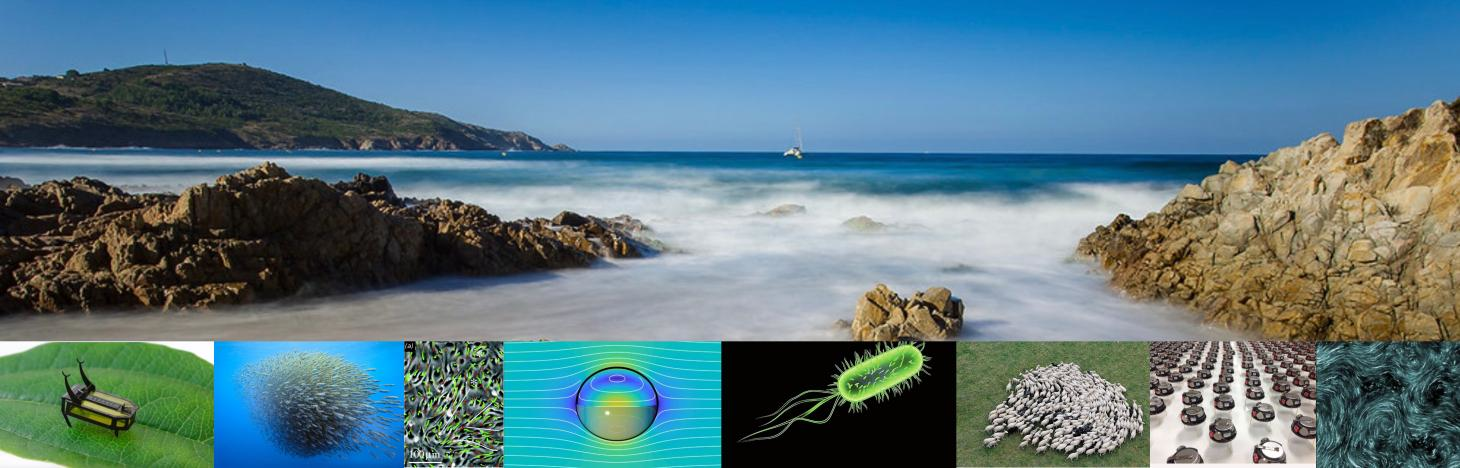
\includegraphics[width = 0.5\columnwidth]{cargese.png}
\caption{This is a sample figure. Can be removed if not needed.\label{figure}}
\end{center}
\end{figure}           


\end{document}


